\chapter{Metodologia}
\label{ch:metodologia}
%Falar porquê do Scrum
%Falar o porquê do Plone

\hspace{2.5cm}

No capítulo de metodologia o objetivo é descrever como ocorreu o processo de construção do sistema, desde a justificativa para a escolha dos métodos de desenvolvimento até a completa entrega do software ao cliente. 

O capítulo está dividido no seguinte escopo: as Seções \ref{sec:defMetodologia} e \ref{sec:defCMS} justificam a escolha da metodologia de desenvolvimento e do Sistema de Gerenciamento de Conteúdo para a implementação do sistema, a Seção \ref{sec:hospedagem-dominio} apresenta uma análise de custos para contratação de planos de hospedagem e registro de domínio e, por último, a seção \ref{sec:desenvolvimento} apresenta como todas as etapas de implementação e reuniões com o cliente foram estabelecidas.

\hspace{2.5cm}

\section{Definição do tipo de metodologia ágil de desenvolvimento}
\label{sec:defMetodologia}

\hspace{2.5cm}

A definição de uma metodologia ágil de desenvolvimento para o atual projeto é consequência das informações apresentadas na Seção \ref{sec:metodologiaagil}, principalmente em relação às informações levantadas no Quadro \ref{comparativo-metodologias}, no Capítulo \ref{ch:referencial}, que dizem respeito a características das metodologias ágeis e tradicionais, principalmente relativas a tempo, comunicação e riscos tendo em vista a baixa complexidade do projeto, o curto tempo para desenvolvimento e produção da documentação.

Após a certificação de que uma metodologia ágil deve ser empregada, pode-se dizer que vários são os motivos para a escolha do \textit{Scrum} como metodologia de desenvolvimento e \citeonline[~p. 560]{Vasconcelos2015} divulga diversos deles em seu trabalho. Pode-se citar a diminuição de reclamações \apud{mann2005case}{Vasconcelos2015}, o aumento do retorno do investimento em projetos de novos produtos \apud{sulaiman2006agileevm}{Vasconcelos2015}, a melhoria da qualidade do produto produzido e diminuição dos custos de produção \apud{sutherland2008fully}{Vasconcelos2015} e a diminuição no tempo gasto para terminar projetos de desenvolvimento de novos produtos \apud{sanders2007using}{Vasconcelos2015}.

Três características pertencentes ao \textit{Scrum} são a leveza, a simplicidade de entender e a dificuldade de se dominá-lo \apud{sutherland2007scrum}{painka12013utilizaccao}, isto porque é fácil entender suas etapas e o papel de cada um no projeto, mas para adequar essa metodologia à realidade da empresa é necessário experiência e conhecimento.

Assim, às vezes pode ser conveniente alterar prazos, papéis e etapas da metodologia, visando torná-la uma ferramenta de auxílio customizada, e fatores como a disponibilidade de clientes, curtos prazos ou complexidade das tarefas devem interferir em decisões dessa espécie, por isso cada projeto utiliza o \textit{Scrum} de uma maneira, ficando a critério das equipes, em especial o \textit{Scrum Master}, quando e onde remodelar.

Outros fatores que contribuiram para definição do \textit{Scrum} como metodologia de desenvolvimento para o projeto atual estão esclarecidos na Tabela \ref{scrumVSxp} e são alusivos ao tamanho da equipe, que corresponde a uma única pessoa, e à elicitação de requisitos, que, por sua vez, não possui uma única forma de ser elaborada. Também contribui para o processo de definição a familiaridade do autor com a metodologia mencionada, já tendo sido estudada e colocada em prática em situações ocorridas durante o curso de Sistemas de Informação.


\hspace{2.5cm}
\section{Definição do Sistema de Gerenciamento de Conteúdo}
\label{sec:defCMS}

\hspace{2.5cm}

Analisando as informações extraídas na Subseção \ref{subsec:comparacao}, no Capítulo \ref{ch:referencial}, o sistema para gerenciamento de conteúdo escolhido pelo autor foi o \textit{Plone}. Os principais fatores que influenciaram nesta decisão estão atrelados ao desempenho e segurança de \textit{websites} construídos com esse CMS. Também é importante destacar que o \textit{Plone} é bastante usado para criação de portais, por exemplo o portal da UFVJM, que possuem características semelhantes ao sistema da Kuruatuba, como a publicação de notícias e eventos. 

Em seu site oficial, \citeonline{plone-org} cita grandes instituições de ensino que utilizam o gerenciador \textit{Plone}, tais como: Universidade Nacional de Córdoba, na Argentina; Universidade da Califórnia Los Angeles (UCLA), no Estados Unidos; e Universidade de Koblenz and Landau, na Alemanha. Como o \textit{Plone} funciona de forma integrada ao \textit{Zope} sua segurança se torna um aspecto positivo, visto que, dentre seus principais recursos, a combinação \textit{Zope}/\textit{Plone} utiliza uma arquitetura de 3 camadas para comunicação interna de seus componentes, separando-os de acordo com suas atribuições no sitema \cite{pastore}. 

O \textit{Plone} possui ferramentas personalizadas e de fácil manipulação que facilitam o gerenciamento de notícias e eventos, primeiramente por possuir campos e opções já pré definidos para o tipo de conteúdo que o usuário irá inserir, e por último por inserir automaticamente o conteúdo criado na lista de conteúdos, devido a uma configuração realizada somente uma vez ao criar o sistema. Sendo assim, basta que o usuário preencha os dados relacionados ao tipo de conteúdo (notícia ou evento) para que ele seja criado e já exibido na página web.

Outro ponto positivo do \textit{Plone} é que sua utilização não necessita da instalação de \textit{plug-ins}, extensões ou complementos, podendo ter seus elementos estáticos, como rodapé e cabeçalho, personalizados via \textit{Portlets}, que segundo \citeonline{UFRGS2012}, são aplicativos e ferramentas prontas para uso em qualquer instalação padrão, podendo ser usadas para calendário, notícias, eventos, menu de busca, enquetes, etc. 

\hspace{2.5cm}
\section{Análise de custos sobre hospedagem e domínio}
\label{sec:hospedagem-dominio}
\hspace{2.5cm}

Uma etapa importante na construção de um ou mais sistemas para uma organização sem fins lucrativos é a contratação de serviços de hospedagem e registro de domínio, isto porque é essencial minimizar os custos mantendo, porém, a qualidade desses serviços. Com o propósito de escolher as empresas provedoras dos serviços de hospedagem e registro de domínio, esta seção apresentará um breve comparativo entre os planos de algumas empresas que atuam na prestação desses serviços.

Para o registro de domínio, foram consultados os preços estipulados por quatro das empresas mais conhecidas nesse ramo, são elas: GoDaddy, Hostgator, Locaweb e Hostinger. Para o domínio \textit{http://www.kuruatuba.org}, os valores encontrados estão na Tabela \ref{comparativo-dominio}. 

\begin{table}[h]
\centering
\scalefont{0.8}
\caption{Preços cobrados pelas empresas para registro do domínio}
\vspace{0.5cm}

\setlength{\extrarowheight}{0.15cm}
\begin{tabular}{l|c}
 
\textbf{Empresa} & \textbf{Valor (R\$/ano)} \\ % Note a separação de col. e a quebra de linhas
\hline                               % para uma linha horizontal
GoDaddy & 49,99 \\
Hostgator & 49,99 \\
Locaweb & 36,90 \\
Hostinger & 59 \\

\hline   
\end{tabular}
\fonte{Autor.}
\label{comparativo-dominio}
\end{table}

Como a única variável a ser analisada para a escolha da empresa é o valor cobrado pelo registro, a empresa contratada para registrar o domínio do portal da Kuruatuba foi a Locaweb, que elaborou um orçamento com custo inferior às demais. 

A escolha da hospedagem a ser utilizada é possivelmente mais complexa e então necessita uma análise maior por parte do responsável pelo desenvolvimento. Tal complexidade se justifica pela quantidade de variáveis a serem consideradas, como: capacidade de armazenamento e tamanho da largura de banda, e pelo valor médio para contratação de uma VPS, que, por sua vez, é maior que o valor médio de uma hospedagem compartilhada.

Embora haja maior complexidade na análise, algumas opções encontradas no mercado de hospedagem de \textit{websites} foram descartadas rapidamente porque seus planos se aproximam da realidade de empresas maiores, que necessitam utilizar muitos recursos e em alta velocidade tanto para clientes quanto para seus próprios funcionários e estão dispostas a pagar mais pelo serviço. 

Após pesquisas de preços para hopedagem de VPS, foram encontradas duas empresas que possuem um plano básico que se adequa à realidade da Kuruatuba: a Hostinger e a DokeHost. As especificações ou variáveis consideradas que mais se diferem e importam para a hospedagem do portal e do sistema da Kuruatuba foram as seguintes: capacidade de aórmazenamento da memória RAM, capacidade de processamento, capacidade de armazenamento da memória secundária e o preço para contratação do serviço. O comparativo das empresas em relação a essas especificações está representada na Tabela \ref{comparativo-hospedagem}.

\newpage

\begin{table}[h]
\centering
\scalefont{0.8}
\caption{Comparativo entre os planos de hospedagem}
\vspace{0.5cm}

\setlength{\extrarowheight}{0.15cm}
\begin{tabular}{l|c|c|c|c}
 
\textbf{Empresa} & \textbf{Memória RAM} & \textbf{vCPU (Quantidade de núcleos)} & \textbf{Memória secundária} & \textbf{Valor (R\$/ano)} \\ % Note a separação de col. e a quebra de linhas
\hline                               % para uma linha horizontal
Hostinger & 1GB & 1 & 20GB SSD & 203,88 \\
DokeHost & 1GB & 2 & 30GB SSD & 310,80  \\ 

\hline   
\end{tabular}
\fonte{Autor.}
\label{comparativo-hospedagem}
\end{table}

Com o auxílio de uma máquina virtual, foi realizada uma avaliação sobre os prováveis requerimentos mínimos dos sistemas e as especificações ofertadas em cada um dos planos. Após a avaliação, chegou-se à conclusão que provavelmente não será necessário mais que 20GB de armazenamento e muito menos de um processador de 2 núcleos, dada a simplicidade das aplicações a serem hospedadas. Sabendo que as configurações de servidor mais baratas atendem às necessidades, a empresa contratada para a hospedagem das aplicações foi a Hostinger.   

\hspace{2.5cm}
\section{Desenvolvimento}
\label{sec:desenvolvimento}

\hspace{2.5cm}
%Definir as etapas 
%Levantamento de requisitos (histórias de usuário) - construção das sprints - Casos de uso e fluxos alternativos

A seção de desenvolvimento sinaliza o início, de fato, da realização das tarefas e demais atividades relacionadas à construção do sistema da Kuruatuba. É a partir desse momento que serão informados dados como domínio, hospedagem, requisitos, versões das tecnologias utilizadas e descrição das atividades desempenhadas.

Para o projeto, foram utilizadas as seguintes ferramentas e suas respectivas versões: \textit{Plone} 4.3.18, PHP 8.0, \textit{MySQL} 5.7, \textit{Docker} 19.03.5 e \textit{Git} 2.17.1, este utilizado para o versionamento de código do sistema para cadastro de associados uma vez que ele poderá ser necessário, futuramente, a outro desenvolvedor para atualizações. 

Também é importante mencionar a utilização do \textit{Google Analytics}, que, como já descrito na Seção \ref{sec:ferramentas}, possibilita contabilizar número de visitantes e obter informações sobre eles, como: origem, páginas visitadas e tempo por sessão. Outra informação relevante é a utilização das imagens do \textit{Docker}: \textit{ubuntu/apache2}, \textit{mysql:5.7} e \textit{lmatos/plonebr-zeo}, todas disponíveis no repositório oficial do \textit{Docker}, o \textit{Docker Hub}. 

A escolha da última imagem citada se justifica pela grande customização dos complementos utilizados em portais do governo brasileiro que utilizam a Identidade Digital do Governo (IDG) 2.0, o que facilita muito o trabalho do gerenciador do portal, tornando o \textit{Plone} ainda mais amigável para usuários que desejem adicionar, editar ou excluir elementos rapidamente. Para exemplificar tais complementos pode-se mencionar a capa, que possibilita criar páginas compostas por vários tipos de elementos, sendo muito simples a definição de seu \textit{layout} e inserção dos elementos na mesma.  

A seguir, no decorrer da seção, os temas levantados serão os que se seguem: as Subseções \ref{subsec:historias} e \ref{subsec:requisitos} tratarão da elaboração das histórias de usuário e da coleta de requisitos, respectivamente, a Subseção \ref{subsec:usecase} apresentará os casos de uso e fluxos alternativos do sistema como forma de auxiliar no entendimento de seu funcionamento, a Subseção \ref{subsec:sprints} apresentará como ficaram os elementos do \textit{Scrum} aplicados ao contexto do presente trabalho e, por fim, a estrutura final de \textit{containers} do \textit{Docker} será explicada na Subseção \ref{subsec:docker}.

\hspace{2.5cm}
\subsection{Histórias de usuário}
\label{subsec:historias}
\hspace{2.5cm}

Segundo \citeonline{longo2014utilizaccao} as histórias de usuário são muito importantes tanto para a criação de requisitos nos métodos ágeis \textit{Extreme Programming} e \textit{Scrum} quanto para provocar o envolvimento do cliente, porém \citeonline{carvalho2014proposta} ressaltam que elas não poderão substituir a comunicação entre clientes e equipe.

Cada história de usuário deve conter três expressões: ``como um... '', que identifica o papel do usuário na história; ``eu quero...'', funcionalidades requisitadas; e ``de modo que...'', benefício conquistado ao realizar a tarefa \apud{cohn2004user}{longo2014utilizaccao}; além de seis atributos indispensáveis identificados pelo acrônimo inglês INVEST (\textit{Independent, Negotiable, Valuable to users or customers, Estimatable, Small and Testable}) \cite{cohn2004user} e explicados em \citeonline{carvalho2014proposta}:

\begin{itemize}
 \item Independente: uma história deve poder ser desenvolvida, testada e entregue de forma isolada, uma não depende de outras;
 
 \item Negociável: através das histórias é possível discutir requisitos, e por elas ainda deve haver possibilidade de mudanças de funcionalidades e datas de entrega; 
 
 \item Valoroso: assim como os métodos ágeis as histórias de usuário devem proporcionar valor para o cliente, através delas é importante que sinta satisfação e sentimento de realização com as informações discutidas;
 
 \item Estimável: uma equipe deve ser capaz de definir o nível de complexidade, a mão de obra necessária e o tempo para conseguir implementar uma história de usuário. Caso isso não seja possível a história deve ser dividida em histórias menores até que a estimativa seja validada.
 
 \item Tamanho pequeno: as histórias devem ser pequenas para prover maior agilidade na implementação.
 
 \item Testável: testes devem ser realizados em cada história criada pois além dos conteúdos ficarem mais organizados a equipe também conseguirá codificar cada uma caso os testes sejam aceitos.
 
\end{itemize}

A seguir estão as histórias de usuário para o trabalho em questão já testadas e validadas junto ao cliente, uma observação a ser feita corresponde ao fato de que os nomes utilizados nas histórias são fictícios, não fazendo alusão ou referência a nenhum dos envolvidos.

\textbf{História 1}: Como o presidente da associação, João deseja cadastrar e remover, via computador ou \textit{smartphone}, usuários do sistema que vão contribuir nas divulgações e no gerenciamento de associados, de modo a estabelecer possíveis trocas de contribuidores.

\textbf{História 2}: Como presidente da associação, João também deseja publicar, via computador ou \textit{smartphone}, eventos e notícias e alterar o conteúdo estático das páginas quando for necessário, com o objetivo de executar tais tarefas sem necessitar de outro encarregado a prestar tais serviços.

\textbf{História 3}: Como presidente da associação, João precisa gerenciar, via computador ou \textit{smartphone}, o cadastramento de associados, possibilitando o cadastro, a edição, a remoção, a pesquisa e o fornecimento de carteirinha associativa aos mesmos, com o objetivo de adiantar a realização de tarefas sem necessitar de seus subordinados ou responder à solicitação de colaboradores ou visitantes.

\textbf{História 4}: Como um secretário da associação, Paulo pretende publicar, via computador ou \textit{smartphone}, eventos e notícias e alterar o conteúdo de páginas conforme solicitação de seu superior. 

\textbf{História 5}: Como uma secretária da associação, Maria pretende gerenciar, via computador ou \textit{smartphone}, o cadastramento de associados, possibilitando o cadastro, a edição, a remoção, a pesquisa e o fornecimento de carteirinha associativa aos mesmos de acordo com as solicitações vindas do presidente ou dos próprios associados, no âmbito da geração da carteirinha.

\hspace{2.5cm}
\subsection{Coleta de requisitos}
\label{subsec:requisitos}
\hspace{2.5cm}

Uma etapa extremamente importante no desenvolvimento de produtos é a coleta de requisitos, pois é com base nela que artefato será construído, tendo em vista que este é o momento em que o cliente tenta exprimir o que deseja que o software tenha e seja capaz de processar, envolvendo também a abstração dessas informações pela equipe responsável por passá-las para o desenvolvimento. 

Para que tudo ocorra da melhor maneira a qualidade na comunicação é essencial e uma abordagem superficial das ideias deve ser evitada a fim de eliminar falsas convicções, ideias distintas entre cliente e desenvolvedor e desperdício de tempo e demais recursos. Para isso existem as maneiras de extrair os requisitos de sistema do cliente e usuário, como explanado no tópico de especificação de software, na Seção \ref{sec:engenhariaweb}. Dentre as opções lá citadas e as histórias de usuário particularizadas na Subseção \ref{subsec:historias}, a coleta de requisitos para a aplicação web da Kuruatuba consistiu-se em um formulário e em curtas reuniões com o atual presidente da associação, o professor Erinaldo. 

O formulário, disponibilizado no apêndice \ref{ch:coleta-requisitos}, foi acessível para os futuros utilizadores do sistema para que opinassem sobre o que deveria e o que não deveria estar no produto final, além do grau de importância de cada requisito de acordo com suas exigências e necessidades. De acordo com as respostas registradas no formulário, com reuniões anteriormente mencionadas e com as histórias de usuário descritas obteve-se os seguintes requisitos de sistema:

\begin{enumerate}
 \item sistema de \textit{login} e cadastro para os usuários;
 \item publicação de notícias, eventos e mais informações sobre a associação;
 \item cadastro, atualização e remoção de associados;
 \item sistema para gerar carteirinha para associados;
 \item formulário para receber mensagens dos visitantes; e
 \item \textit{link} para baixar importantes documentos da Kuruatuba.
\end{enumerate}


\hspace{2.5cm}
\subsection{Casos de uso e fluxos de eventos}
\label{subsec:usecase}
\hspace{2.5cm}

A presente subseção está dividida em duas partes: a primeira, exposta em \ref{subsubsec:casos-uso}, aborda de maneira geral sobre diagramas de casos de uso e apresenta o diagrama associado ao trabalho em desenvolvimento; e a segunda, encontrada em \ref{subsubsec:fluxos}, demonstra a versão final dos fluxos de eventos dos casos de uso.

\hspace{2.5cm}
\subsubsection{Diagrama de casos de uso}
\label{subsubsec:casos-uso}
\hspace{2.5cm}

O diagrama de casos de uso pertence à Linguagem de Modelagem Unificada (UML) e é comumente utilizado para documentar requisitos de sistema, modelando seu contexto e facilitando seu entendimento por exibí-lo externamente aos desenvolvedores \cite{de2001diagramas}.

Em geral, os diagramas de casos de uso apresentam os seguintes elementos \cite{zapata2007conversion}:

\begin{itemize}
 \item Casos de uso: ações realizadas pelos atores associados que descrevem do início ao fim do processo;
 \item Atores: são os usuários, sendo humanos ou outros sistemas, que poderão realizar os casos de uso e as funcionalidades do sistema;
 \item Relacionamentos: são interações entre dois casos de uso, dois atores ou um caso de uso e um ator. Elas podem der divididas em quatro tipos:
 
 \begin{enumerate}
  \item associação: estabelece relação entre um ator e um caso de uso;
  \item \textit{include}: inclui o comportamento de um caso de uso em outro, ou seja, ao realizar um caso de uso o outro ligado por meio do \textit{include} também será realizado;
  \item \textit{extend}: a presença do \textit{extend} ligando um caso de uso A a um caso de uso B significa que através de A o \textit{use case} B poderá ser realizado também. Diferentemente do relacionamento anterior, um caso de uso não é obrigatoriamente executado quando o outro for, tal ocorrência se dará por meio de condições; e
  \item herança: este relacionamento simboliza o compartilhamento das especificações de um ator a outro, ou seja, um ator irá herdar todas as permissões em realizar os casos de uso do outro relacionado.
 \end{enumerate}
 
\item Cenário: uma sequência de ações que ilustra um comportamento. São usados para ilustrar a interação ou execução de uma instância a um caso de uso \cite[~p. 239, tradução nossa]{zapata2007conversion}. 

\end{itemize}

Após a breve explicação sobre os diagramas de casos de uso, sua importância e seus elementos, ficam representados nas Figuras \ref{use-case-portal} e \ref{use-case-sistema} os diagramas referentes, respectivamente, ao portal e ao sistema de associados da associação Kuruatuba.


\begin{figure}[htb]
 \centering
 \caption{Diagrama de casos de uso do portal da Kuruatuba}
 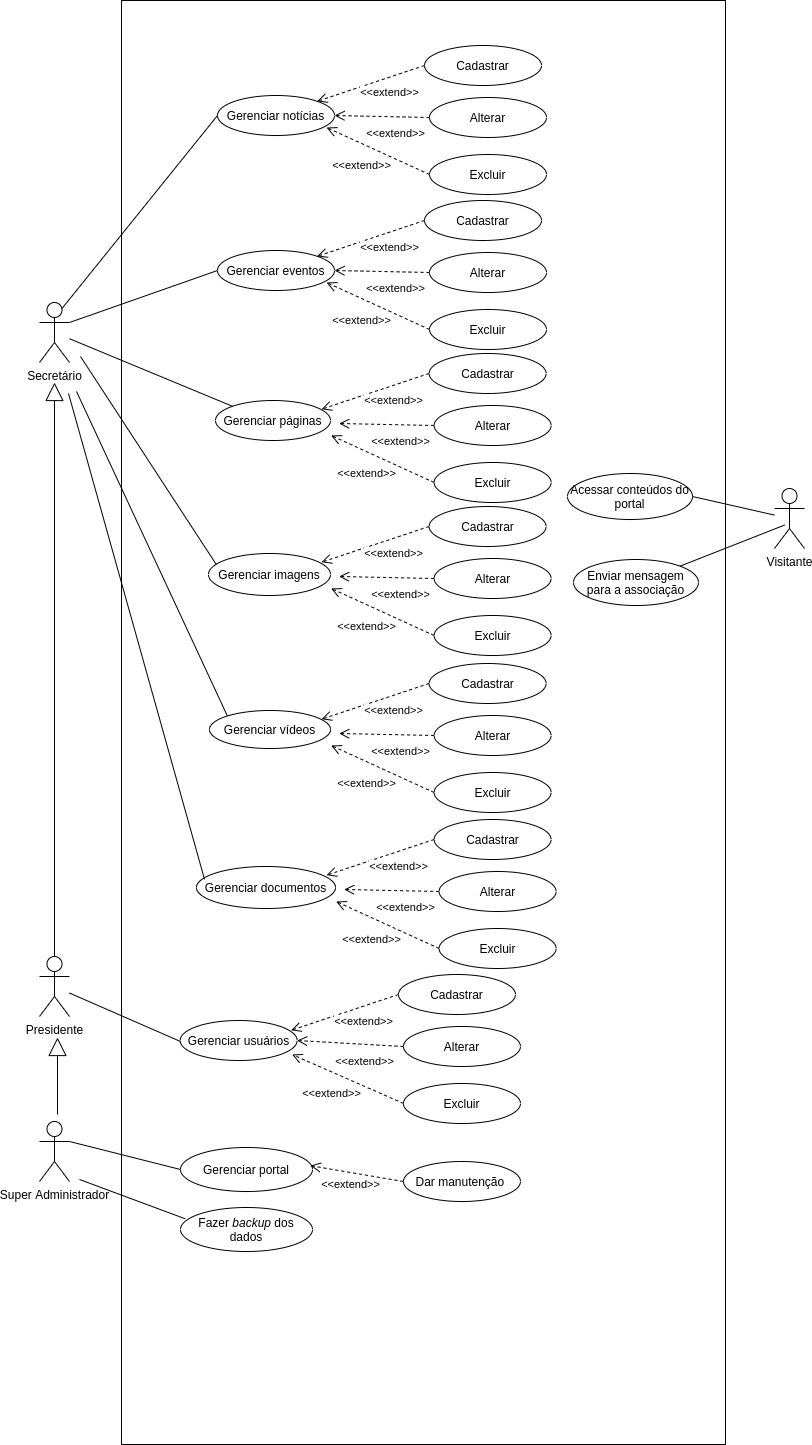
\includegraphics[width=0.8\textwidth]{figuras/use-case-portal.png}
 
 \label{use-case-portal}
 \fonte{Autor.}
\end{figure}

Ao analisar o diagrama anterior, é possível entender que os elementos-chave dos casos de uso são: notícias, eventos, páginas, arquivos de mídia e documentos, usuários, a aplicação ao todo e seus dados, informações que se diferem das presentes no diagrama apresentado na Figura \ref{use-case-sistema}, que se trata sobre o sistema de associados. 

O que se deve absorver e compreender da Figura \ref{use-case-portal} é que os níveis de usuário são distintos de acordo com a importância dos dados a serem manipulados. Por exemplo: as informações gerenciadas pelo presidente e que não são pelos secretários, que são os dados dos usuários do portal, são de extrema importância e necessitam acesso restrito para consulta e modificação. Por isso somente o presidente e o administrador do portal podem gerenciá-los, dada a importância e representatividade de seu cargo na instituição. 

Outra questão importante é a definição de quem exercerá o papel de super administrador. Considerando-se que a associação não possui um agente de Tecnologia da Informação para manipular configurações técnicas do sistema, tanto para a realização de \textit{backup} quanto para a customização do portal e do sistema, foi decidido que o próprio desenvolvedor de ambas aplicações seria responsável por executar tais funções e, por isso, exercerá o papel de super administrador, trabalhando de forma ética e profissional para o bem da instituição.

\begin{figure}[htb]
 \centering
 \caption{Diagrama de casos de uso do sistema de associados da Kuruatuba}
 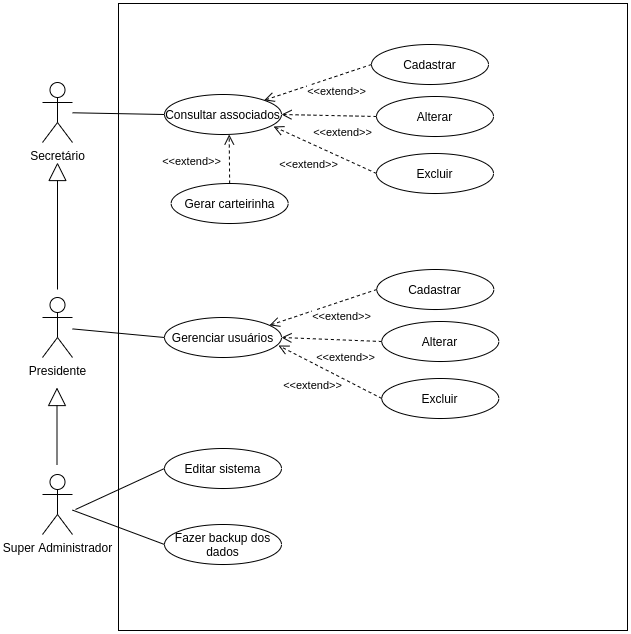
\includegraphics[width=0.8\textwidth]{figuras/use-case-sistema.png}
 
 \label{use-case-sistema}
 \fonte{Autor.}
\end{figure}

Sendo consideravelmente mais simples que o visto anteriormente, o diagrama representado na Figura \ref{use-case-sistema} é de simples compreensão graças ao pequeno número de casos de uso presentes. Pode-se considerar que relação de atribuições entre os atores secretário,  presidente e super administrador é a mesma, visto que o que muda em relação ao nível de usuário é a autorização de cadastrar, editar e excluir usuário do sistema, que não é previsto para o secretário, e a edição (customização) do sistema e realização de \textit{backup}, por sua vez previsto somente para o super administrador, por envolver questões mais técnicas.

\hspace{2.5cm}
\subsubsection{Fluxos de eventos}
\label{subsubsec:fluxos}
\hspace{2.5cm}

A seguir estão os fluxos de eventos para os casos de uso definidos anteriormente. Tais fluxos auxiliam ainda mais na compreensão de como o sistema se comportará após cada requisição do usuário e quais possibilidades de interação com a interface do software este terá ao navegar pelas telas. 

Para o fluxo de eventos do caso de uso ``Gerenciar imagens, vídeos ou documentos'', o termo utilizado para representar todos os três tipos foi ``arquivo'', isto porque, diferentemente dos demais elementos, o \textit{Plone} os trata como arquivos, mesmo tendo suas peculiaridades. Já em relação aos casos de uso ``Dar manutenção'' e ``Fazer backup dos dados'', foi decidido que não serão apresentados seus fluxos de eventos por razões de segurança e complexidade, além de que são etapas só executadas pelo super administrador e com uma frequência ainda não estipulada, embora a ideia inicial é de que sejam executadas com grande intervalo de tempo.  


%criar página
\vspace{0.7cm}
\leftline{ \textbf{Caso de uso}: Criar página.}

\noindent \textit{Pré-condição}: selecionar o botão de salvar.

\noindent \textit{Fluxo principal}:

\begin{enumerate}
    \item selecionar no menu o item ``Conteúdo'';
    \item selecionar no menu o item ``Adicionar item'';
    \item selecionar o item ``Página'';
    \item preencher obrigatoriamente o título; e
    \item selecionar a opção ``Salvar''.
\end{enumerate}

\noindent \textit{Fluxo alternativo}: Cancelamento do cadastro.

\noindent \textit{Pré-condição}: usuário acionou o botão ``Cancelar''.

\noindent \textit{Etapas}:

\begin{enumerate}
    \item selecionar o botão ``Cancelar''; e
    \item o sistema retorna a mensagem: ``Adicionar Novo Item operação cancelada''.
\end{enumerate}

\noindent \textit{Fluxo alternativo}: Não preenchimento do título.

\noindent \textit{Pré-condição}: usuário acionou o botão ``Salvar'' sem ter inserido o título da página.

\noindent \textit{Etapas}:

\begin{enumerate}
    \item selecionar o botão ``Salvar'';
    \item o sistema retorna a mensagem: ``Existem alguns erros''; e
    \item o campo de título apresenta a seguinte mensagem: ``Dado obrigatório não informado''.
\end{enumerate}



%alterar página
\vspace{0.7cm}
\leftline{ \textbf{Caso de uso}: Alterar página.}

\noindent \textit{Pré-condição}: selecionar a página.

\noindent \textit{Fluxo principal}:

\begin{enumerate}
    \item selecionar no menu o item ``Conteúdo'';
    \item selecionar a página;
    \item selecionar no menu o item ``Edição''; e
    \item após realizar as alterações, ir em salvar.
\end{enumerate}

\noindent \textit{Fluxo alternativo}: Cancelamento de alterações.

\noindent \textit{Pré-condição}: usuário acionou o botão ``Cancelar''.

\noindent \textit{Etapas}:

\begin{enumerate}
    \item selecionar o botão ``Cancelar''; e
    \item o sistema retorna a mensagem: ``Edição cancelada''.
\end{enumerate}


%excluir página
\vspace{0.7cm}
\leftline{ \textbf{Caso de uso}: Excluir página.}

\noindent \textit{Pré-condição}: selecionar a opção de excluir a página.

\noindent \textit{Fluxo principal}:

\begin{enumerate}
    \item selecionar no menu o item ``Conteúdo'';
    \item selecionar a página;
    \item selecionar no ícone representado por uma lixeira no canto superior da tela;
    \item o sistema emitirá a mensagem: ``Você tem certeza de que deseja excluir os itens selecionados?''; e
    \item selecionar o botão de confirmação da ação.
\end{enumerate}

\noindent \textit{Fluxo alternativo}: Cancelamento da exclusão.

\noindent \textit{Pré-condição}: usuário acionou o botão ``Não''.

\noindent \textit{Etapas}:

\begin{enumerate}
    \item selecionar o botão ``Não''.
\end{enumerate}


%cadastrar notícia
\vspace{0.7cm}
\leftline{ \textbf{Caso de uso}: Publicar notícia.}

\noindent \textit{Pré-condição}: selecionar a opção de salvar a notícia.

\noindent \textit{Fluxo principal}:

\begin{enumerate}
    \item selecionar no menu o item ``Conteúdo'';
    \item selecionar a pasta notícias;
    \item selecionar a pasta do ano da notícia;
    \item selecionar no menu o item ``Adicionar item'';
    \item selecionar o item ``Notícia'';
    \item preencher obrigatoriamente o título;
    \item selecionar a opção ``Salvar'';
    \item selecionar no menu o item ``Estado''; e
    \item selecionar a opção ``Publicar''.
\end{enumerate}

\noindent \textit{Fluxo alternativo}: Cancelamento do cadastro.

\noindent \textit{Pré-condição}:  usuário acionou o botão ``Cancelar''.

\noindent \textit{Etapas}:

\begin{enumerate}
    \item selecionar o botão ``Cancelar''; e
    \item o sistema retorna a mensagem: ``Adicionar Novo Item operação cancelada''.
\end{enumerate}

\noindent \textit{Fluxo alternativo}: Não preenchimento do título.

\noindent \textit{Pré-condição}: usuário acionou o botão ``Salvar'' sem ter inserido o título da notícia.

\noindent \textit{Etapas}:

\begin{enumerate}
    \item selecionar o botão ``Salvar'';
    \item o sistema retorna a mensagem: ``Existem alguns erros''; e
    \item o campo de título apresenta a seguinte mensagem: ``Dado obrigatório não informado''.
\end{enumerate}




%editar notícia
\vspace{0.7cm}
\leftline{ \textbf{Caso de uso}: Alterar notícia.}

\noindent \textit{Pré-condição}: selecionar a opção de editar a notícia.

\noindent \textit{Fluxo principal}:

\begin{enumerate}
    \item selecionar no menu o item ``Conteúdo'';
    \item selecionar a pasta notícias;
    \item selecionar a pasta do ano da notícia;
    \item selecionar a notícia; e
    \item selecionar no menu o item ``Edição''.
\end{enumerate}

\noindent \textit{Fluxo alternativo}: Cancelamento da edição.

\noindent \textit{Pré-condição}: usuário acionou o botão ``Cancelar''.

\noindent \textit{Etapas}:

\begin{enumerate}
    \item selecionar o botão ``Cancelar''; e
    \item o sistema retorna a mensagem: ``Edição cancelada''.
\end{enumerate}

\noindent \textit{Fluxo alternativo}: Não preenchimento do título.

\noindent \textit{Pré-condição}: usuário acionou o botão ``Salvar'' sem ter inserido o título da notícia.

\noindent \textit{Etapas}:

\begin{enumerate}
    \item selecionar o botão ``Salvar'';
    \item o sistema retorna a mensagem: ``Existem alguns erros''; e
    \item o campo de título apresenta a seguinte mensagem: ``Dado obrigatório não informado''.
\end{enumerate}




%excluir notícia
\vspace{0.7cm}
\leftline{ \textbf{Caso de uso}: Excluir notícia.}

\noindent \textit{Pré-condição}: selecionar a opção de excluir a notícia.

\noindent \textit{Fluxo principal}:

\begin{enumerate}
    \item selecionar no menu o item ``Conteúdo'';
    \item selecionar a pasta notícias;
    \item selecionar a pasta do ano da notícia;
    \item selecionar a notícia;
    \item selecionar no menu o item ``Ações'';
    \item ir em ``Excluir'';
    \item o sistema emitirá a mensagem: ``Você realmente quer apagar este item?''; e
    \item selecionar a opção de excluir.
\end{enumerate}

\noindent \textit{Fluxo alternativo}: Cancelamento da exclusão.

\noindent \textit{Pré-condição}: usuário acionou o botão ``Cancelar''.

\noindent \textit{Etapas}:

\begin{enumerate}
    \item selecionar o botão ``Cancelar''.
\end{enumerate}


%cadastrar evento
\vspace{0.7cm}
\leftline{ \textbf{Caso de uso}: Publicar evento.}

\noindent \textit{Pré-condição}: selecionar a opção de salvar o evento.

\noindent \textit{Fluxo principal}:

\begin{enumerate}
    \item selecionar no menu o item ``Conteúdo'';
    \item selecionar a pasta eventos;
    \item selecionar a pasta do ano do evento;
    \item selecionar no menu o item ``Adicionar item'';
    \item selecionar o item ``Evento'';
    \item preencher obrigatoriamente o título;
    \item selecionar a opção ``Salvar'';
    \item selecionar no menu o item ``Estado''; e
    \item selecionar a opção ``Publicar''.
\end{enumerate}

\noindent \textit{Fluxo alternativo}: Cancelamento do cadastro.

\noindent \textit{Pré-condição}:  usuário acionou o botão ``Cancelar''.

\noindent \textit{Etapas}:

\begin{enumerate}
    \item selecionar o botão ``Cancelar''; e
    \item o sistema retorna a mensagem: ``Adicionar Novo Item operação cancelada''.
\end{enumerate}

\noindent \textit{Fluxo alternativo}: Não preenchimento do título.

\noindent \textit{Pré-condição}: usuário acionou o botão ``Salvar'' sem ter inserido o título do evento.

\noindent \textit{Etapas}:

\begin{enumerate}
    \item selecionar o botão ``Salvar'';
    \item o sistema retorna a mensagem: ``Existem alguns erros''; e
    \item o campo de título apresenta a seguinte mensagem: ``Dado obrigatório não informado''.
\end{enumerate}



%editar evento
\vspace{0.7cm}
\leftline{ \textbf{Caso de uso}: Alterar evento.}

\noindent \textit{Pré-condição}: selecionar a opção de editar o evento.

\noindent \textit{Fluxo principal}:

\begin{enumerate}
    \item selecionar no menu o item ``Conteúdo'';
    \item selecionar a pasta eventos;
    \item selecionar a pasta do ano do evento;
    \item selecionar o evento; e
    \item selecionar no menu o item ``Edição''.
\end{enumerate}

\noindent \textit{Fluxo alternativo}: Cancelamento da edição.

\noindent \textit{Pré-condição}: usuário acionou o botão ``Cancelar''.

\noindent \textit{Etapas}:

\begin{enumerate}
    \item selecionar o botão ``Cancelar''; e
    \item o sistema retorna a mensagem: ``Edição cancelada''.
\end{enumerate}

\noindent \textit{Fluxo alternativo}: Não preenchimento do título.

\noindent \textit{Pré-condição}: usuário acionou o botão ``Salvar'' sem ter inserido o título do evento.

\noindent \textit{Etapas}:

\begin{enumerate}
    \item selecionar o botão ``Salvar'';
    \item o sistema retorna a mensagem: ``Existem alguns erros''; e
    \item o campo de título apresenta a seguinte mensagem: ``Dado obrigatório não informado''.
\end{enumerate}



%excluir evento
\vspace{0.7cm}
\leftline{ \textbf{Caso de uso}: Excluir evento.}

\noindent \textit{Pré-condição}: selecionar a opção de excluir o evento.

\noindent \textit{Fluxo principal}:

\begin{enumerate}
    \item selecionar no menu o item ``Conteúdo'';
    \item selecionar a pasta eventos;
    \item selecionar a pasta do ano do evento;
    \item selecionar o evento;
    \item selecionar no menu o item ``Ações'';
    \item ir em ``Excluir'';
    \item o sistema emitirá a mensagem: ``Você realmente quer apagar este item?''; e
    \item selecionar a opção de excluir.
\end{enumerate}

\noindent \textit{Fluxo alternativo}: Cancelamento da exclusão.

\noindent \textit{Pré-condição}: usuário acionou o botão ``Cancelar''.

\noindent \textit{Etapas}:

\begin{enumerate}
    \item selecionar o botão ``Cancelar''.
\end{enumerate}



%cadastrar arquivo
\vspace{0.7cm}
\leftline{ \textbf{Caso de uso}: Cadastrar arquivo.}

\noindent \textit{Pré-condição}: selecionar a opção de adicionar arquivo ou adicionar imagem.

\noindent \textit{Fluxo principal}:

\begin{enumerate}
    \item selecionar no menu o item ``Conteúdo'';
    \item selecionar a pasta onde deseja adicionar o arquivo;
    \item selecionar no menu o item ``Adicionar arquivo'';
    \item anexar obrigatoriamente o arquivo;
    \item selecionar a opção ``Salvar'';
    \item sistema retorna a mensagem: ``item criado''.
\end{enumerate}

\noindent \textit{Fluxo alternativo}: Cancelamento do cadastro.

\noindent \textit{Pré-condição}:  usuário acionou o botão ``Cancelar''.

\noindent \textit{Etapas}:

\begin{enumerate}
    \item selecionar o botão ``Cancelar''; e
    \item o sistema leva o usuário até o diretório onde estava.
\end{enumerate}



%editar arquivo
\vspace{0.7cm}
\leftline{ \textbf{Caso de uso}: Alterar arquivo.}

\noindent \textit{Pré-condição}: selecionar a opção de editar o arquivo.

\noindent \textit{Fluxo principal}:

\begin{enumerate}
    \item selecionar no menu o item ``Conteúdo'';
    \item selecionar a pasta do arquivo;
    \item selecionar o arquivo; e
    \item selecionar no menu o item ``Edição''.
\end{enumerate}

\noindent \textit{Fluxo alternativo}: Cancelamento da edição.

\noindent \textit{Pré-condição}: usuário acionou o botão ``Cancelar''.

\noindent \textit{Etapas}:

\begin{enumerate}
    \item selecionar o botão ``Cancelar''; e
    \item o sistema retorna a mensagem: ``Edição cancelada''.
\end{enumerate}


%excluir arquivo
\vspace{0.7cm}
\leftline{ \textbf{Caso de uso}: Excluir arquivo.}

\noindent \textit{Pré-condição}: selecionar a opção de excluir o arquivo.

\noindent \textit{Fluxo principal}:

\begin{enumerate}
    \item selecionar no menu o item ``Conteúdo'';
    \item selecionar a pasta do arquivo;
    \item selecionar o arquivo;
    \item selecionar no menu o item ``Ações'';
    \item ir em ``Excluir'';
    \item o sistema emitirá a mensagem: ``Você realmente quer apagar este item?''; e
    \item selecionar a opção de excluir.
\end{enumerate}

\noindent \textit{Fluxo alternativo}: Cancelamento da exclusão.

\noindent \textit{Pré-condição}: usuário acionou o botão ``Cancelar''.

\noindent \textit{Etapas}:

\begin{enumerate}
    \item selecionar o botão ``Cancelar''.
\end{enumerate}



%Gerenciar usuários
\vspace{0.7cm}
\leftline{ \textbf{Caso de uso}: Consultar usuários.}

\noindent \textit{Pré-condição}: estar na página de usuários.

\noindent \textit{Fluxo principal}:

\begin{enumerate}
    \item selecionar no menu o item ``Configuração de site''; e
    \item selecionar a opção ``Usuários e grupos''.
\end{enumerate}

\noindent \textit{Fluxo alternativo}: não se aplica.



%cadastrar usuário
\vspace{0.7cm}
\leftline{ \textbf{Caso de uso}: Cadastrar usuário.}

\noindent \textit{Pré-condição}: selecionar o botão ``Registrar''.

\noindent \textit{Fluxo principal}:

\begin{enumerate}
    \item selecionar no menu o item ``Configuração de site'';
    \item selecionar a opção ``Usuários e grupos'';
    \item selecionar o botão ``Adicionar Novo Usuário'';
    \item informar, obrigatoriamente, e-mail e nome de usuário; e
    \item selecionar o botão de registrar o usuário.
\end{enumerate}

\noindent \textit{Fluxo alternativo}: Não preenchimento de e-mail ou nome de usuário.

\noindent \textit{Pré-condição}: usuário acionou o botão ``Registrar'' sem ter inserido o e-mail ou nome de usuário.

\noindent \textit{Etapas}:

\begin{enumerate}
    \item selecionar o botão ``Registrar'';
    \item o sistema retorna a mensagem: ``Houve erros''; e
    \item os campos de e-mail e usuário apresentam a seguinte mensagem: ``Dado obrigatório não informado''.
\end{enumerate}


%alterar usuário
\vspace{0.7cm}
\leftline{ \textbf{Caso de uso}: Alterar usuário.}

\noindent \textit{Pré-condição}: selecionar o botão ``Salvar''.

\noindent \textit{Fluxo principal}:

\begin{enumerate}
    \item selecionar no menu o item ``Configuração de site'';
    \item selecionar a opção ``Usuários e grupos'';
    \item preencher o campo ``Busca de Usuários'';
    \item selecionar o nome do usuário requisitado;
    \item preencher substituir as informações dos campos necessários; e
    \item acessar o botão de salvar as informações.
\end{enumerate}

\noindent \textit{Fluxo alternativo}: Cancelamento da edição.

\noindent \textit{Pré-condição}: usuário acionou o botão ``Cancelar''.

\noindent \textit{Etapas}:

\begin{enumerate}
    \item selecionar o botão ``Cancelar''; e
    \item sistema exibe a mensagem: ``Alterações canceladas''.
\end{enumerate}

\noindent \textit{Fluxo alternativo}: Não preenchimento do e-mail.

\noindent \textit{Pré-condição}: usuário acionou o botão ``Salvar'' sem ter haver um e-mail inserido.

\noindent \textit{Etapas}:

\begin{enumerate}
    \item o sistema retorna a mensagem: ``Existem alguns erros''; e
    \item o campo de e-mail apresenta a seguinte mensagem: ``Dado obrigatório não informado''.
\end{enumerate}



%remover usuário
\vspace{0.7cm}
\leftline{ \textbf{Caso de uso}: Excluir usuário.}

\noindent \textit{Pré-condição}: selecionar o botão ``Salvar''.

\noindent \textit{Fluxo principal}:

\begin{enumerate}
    \item selecionar no menu o item ``Configuração de site'';
    \item selecionar a opção ``Usuários e grupos'';
    \item preencher o campo ``Busca de Usuários'';
    \item selecionar a caixa ``Remover'' na linha onde se encontra o nome do usuário requisitado; e
    \item selecionar o botão de salvar as informações.
\end{enumerate}

\noindent \textit{Fluxo alternativo}: não se aplica.


%enviar mensagem
\vspace{0.7cm}
\leftline{ \textbf{Caso de uso}: Enviar mensagem para a associação.}

\noindent \textit{Pré-condição}: selecionar o botão ``Enviar''.

\noindent \textit{Fluxo principal}:

\begin{enumerate}
    \item acessar a aba contato;
    \item inserir as informações para a mensagem; e
    \item selecionar o botão de envio.
\end{enumerate}

\noindent \textit{Fluxo alternativo}: Não preenchimento do nome, e-mail, assunto ou corpo da mensagem.

\noindent \textit{Pré-condição}: usuário acionou o botão ``Enviar'' sem ter preenchido nome, e-mail, assunto ou texto da mensagem.

\noindent \textit{Etapas}:

\begin{enumerate}
    \item os campos obrigatórios vazios apresentam a seguinte mensagem: ``Preencha este campo''.
\end{enumerate}

%SISTEMA DE ASSOCIADOS

%consultar associados
\vspace{0.7cm}
\leftline{ \textbf{Caso de uso}: Consultar associados.}

\noindent \textit{Pré-condição}: preencher o campo ``Pesquisar''.

\noindent \textit{Fluxo principal}:

\begin{enumerate}
    \item na página inicial do sistema, inserir alguma informação sobre qualquer atributo do usuário; e
    \item a medida que o usuário digitar, o sistema retornará, em tempo real, os resultados para busca.
\end{enumerate}

\noindent \textit{Fluxo alternativo}: não se aplica.


%consultar associados
\vspace{0.7cm}
\leftline{ \textbf{Caso de uso}: Ver detalhes.}

\noindent \textit{Pré-condição}: selecionar o botão ``Exibir detalhes''.

\noindent \textit{Fluxo principal}:

\begin{enumerate}
    \item na página inicial do sistema, selecionar o botão ``Exibir detalhes'' de um associado; e
    \item o sistema retorna as seguintes informações do associado: número de identificação, nome, apelido, rua, número, bairro, número de telefone/celular, e-mail, número do Registro Geral (RG) e número do Cadastro de Pessoas Físicas (CPF).
\end{enumerate}

\noindent \textit{Fluxo alternativo}: não se aplica.


%cadastrar associado
\vspace{0.7cm}
\leftline{ \textbf{Caso de uso}: Cadastrar associado.}

\noindent \textit{Pré-condição}: selecionar a opção de registrar o associado.

\noindent \textit{Fluxo principal}:

\begin{enumerate}
    \item acionar o botão ``Adicionar Associado'';
    \item preencher obrigatoriamente nome, e-mail identidade, CPF, telefone, rua, número e bairro; e
    \item selecionar o botão ``Registrar Associado''.
\end{enumerate}

\noindent \textit{Fluxo alternativo}: Cancelamento do cadastro.

\noindent \textit{Pré-condição}: usuário acionou o botão ``Voltar''.

\noindent \textit{Etapas}:

\begin{enumerate}
    \item selecionar o botão ``Voltar''.
\end{enumerate}

\noindent \textit{Fluxo alternativo}: Não preenchimento dos dados obrigatórios.

\noindent \textit{Pré-condição}: usuário acionou o botão ``Salvar'' sem ter inserido os dados obrigatórios.

\noindent \textit{Etapas}:

\begin{enumerate}
    \item selecionar o botão ``Salvar''; e
    \item os campos obrigatórios apresentam a seguinte mensagem: ``Preencha este campo''.
\end{enumerate}


\noindent \textit{Fluxo alternativo}: Endereço de e-mail não é válido.

\noindent \textit{Pré-condição}: usuário solicitou cadastrar associado com um e-mail inválido.

\noindent \textit{Etapas}:

\begin{enumerate}
    \item selecionar o botão ``Salvar''; e
    \item sistema retorna a seguinte mensagem: ``E-mail inválido!''.
\end{enumerate}


\noindent \textit{Fluxo alternativo}: CPF não é válido.

\noindent \textit{Pré-condição}: usuário solicitou cadastrar associado com um CPF inválido.

\noindent \textit{Etapas}:

\begin{enumerate}
    \item selecionar o botão ``Salvar''; e
    \item sistema retorna a seguinte mensagem: ``CPF inválido!''.
\end{enumerate}


\noindent \textit{Fluxo alternativo}: Identidade ou CPF já existente na base de dados.

\noindent \textit{Pré-condição}: usuário solicitou cadastrar associado com um número de identidade ou CPF já existente no banco de dados.

\noindent \textit{Etapas}:

\begin{enumerate}
    \item selecionar o botão ``Salvar''; e
    \item sistema retorna a seguinte mensagem: ``CPF ou identidade já existe no sistema!''.
\end{enumerate}


%editar associado
\vspace{0.7cm}
\leftline{ \textbf{Caso de uso}: Alterar associado.}

\noindent \textit{Pré-condição}: selecionar a opção de atualizar o associado.

\noindent \textit{Fluxo principal}:

\begin{enumerate}
    \item selecionar o ícone de edição na linha do registro a ser atualizado;
    \item editar os campos necessários; e
    \item selecionar o botão de atualizar o associado.
\end{enumerate}

\noindent \textit{Fluxo alternativo}: Cancelamento da edição.

\noindent \textit{Pré-condição}: usuário acionou o botão ``Voltar''.

\noindent \textit{Etapas}:

\begin{enumerate}
    \item Selecionar o botão ``Voltar''.
\end{enumerate}

\noindent \textit{Fluxo alternativo}: Não preenchimento dos dados obrigatórios.

\noindent \textit{Pré-condição}: usuário acionou o botão ``Salvar'' sem ter inserido os dados obrigatórios.

\noindent \textit{Etapas}:

\begin{enumerate}
    \item selecionar o botão ``Atualizar Associado''; e
    \item os campos obrigatórios apresentam a seguinte mensagem: ``Preencha este campo''.
\end{enumerate}


\noindent \textit{Fluxo alternativo}: Endereço de e-mail não é válido.

\noindent \textit{Pré-condição}: usuário solicitou atualizar associado com um e-mail inválido.

\noindent \textit{Etapas}:

\begin{enumerate}
    \item selecionar o botão ``Atualizar Associado''; e
    \item sistema retorna a seguinte mensagem: ``E-mail inválido!''.
\end{enumerate}


\noindent \textit{Fluxo alternativo}: CPF não é válido.

\noindent \textit{Pré-condição}: usuário solicitou atualizar associado com um CPF inválido.

\noindent \textit{Etapas}:

\begin{enumerate}
    \item selecionar o botão ``Atualizar Associado''; e
    \item sistema retorna a seguinte mensagem: ``CPF inválido!''.
\end{enumerate}


\noindent \textit{Fluxo alternativo}: Identidade ou CPF já existente na base de dados.

\noindent \textit{Pré-condição}: usuário solicitou atualizar associado com um número de identidade ou CPF já existente no banco de dados.

\noindent \textit{Etapas}:

\begin{enumerate}
    \item selecionar o botão ``Atualizar Associado''; e
    \item sistema retorna a seguinte mensagem: ``CPF ou identidade já existe no sistema!''.
\end{enumerate}



%excluir associado
\vspace{0.7cm}
\leftline{ \textbf{Caso de uso}: Excluir associado.}

\noindent \textit{Pré-condição}: selecionar a opção de excluir o associado.

\noindent \textit{Fluxo principal}:

\begin{enumerate}
    \item selecionar o ícone de exclusão na linha do registro a ser atualizado;
    \item o sistema exibirá uma mensagem de confirmação de exclusão; e
    \item selecionar o botão ``OK''.
\end{enumerate}

\noindent \textit{Fluxo alternativo}: Cancelamento da exclusão.

\noindent \textit{Pré-condição}: usuário acionou o botão ``Cancelar''.

\noindent \textit{Etapas}:

\begin{enumerate}
    \item selecionar o botão ``Cancelar''.
\end{enumerate}


%%Implementar e alterar fluxo
%consultar usuário
\vspace{0.7cm}
\leftline{ \textbf{Caso de uso}: Consultar usuários.}

\noindent \textit{Pré-condição}: preencher o campo ``Pesquisar''.

\noindent \textit{Fluxo principal}:

\begin{enumerate}
    \item na página inicial do sistema, inserir alguma informação sobre qualquer atributo do usuário; e
    \item a medida que o usuário digitar, o sistema retornará, em tempo real, os resultados para busca.
\end{enumerate}

\noindent \textit{Fluxo alternativo}: não se aplica.


%cadastrar usuário
\vspace{0.7cm}
\leftline{ \textbf{Caso de uso}: Cadastrar usuário.}

\noindent \textit{Pré-condição}: selecionar a opção de registrar administrador.

\noindent \textit{Fluxo principal}:

\begin{enumerate}
    \item acionar o botão ``Registrar Administrador'';
    \item preencher nome, e-mail, senha e nível de permissão (secretário ou presidente); e
    \item selecionar o botão ``Registrar Administrador''.
\end{enumerate}

\noindent \textit{Fluxo alternativo}: Cancelamento do cadastro.

\noindent \textit{Pré-condição}: usuário acionou o botão ``Voltar''.

\noindent \textit{Etapas}:

\begin{enumerate}
    \item selecionar o botão ``Voltar''.
\end{enumerate}

\noindent \textit{Fluxo alternativo}: Não preenchimento dos dados obrigatórios.

\noindent \textit{Pré-condição}: usuário acionou o botão ``Salvar'' sem ter inserido os dados obrigatórios.

\noindent \textit{Etapas}:

\begin{enumerate}
    \item selecionar o botão ``Registrar Administrador''; e
    \item os campos obrigatórios apresentam a seguinte mensagem: ``Preencha este campo''.
\end{enumerate}


\noindent \textit{Fluxo alternativo}: Nível de permissão de secretário.

\noindent \textit{Pré-condição}: usuário do tipo ``secretário'' solicitou cadastrar administrador ao sistema.

\noindent \textit{Etapas}:

\begin{enumerate}
    \item selecionar o botão ``Adicionar Administrador''; e
    \item sistema retorna a seguinte mensagem: ``Você não tem permissão para realizar essa operação!''.
\end{enumerate}


\noindent \textit{Fluxo alternativo}: Endereço de e-mail não é válido.

\noindent \textit{Pré-condição}: usuário solicitou cadastrar usuário com um e-mail inválido.

\noindent \textit{Etapas}:

\begin{enumerate}
    \item selecionar o botão ``Registrar Administrador''; e
    \item sistema retorna a seguinte mensagem: ``E-mail inválido!''.
\end{enumerate}


\noindent \textit{Fluxo alternativo}: E-mail já existente na base de dados.

\noindent \textit{Pré-condição}: usuário solicitou cadastrar usuário com um endereço de e-mail já existente no banco de dados.

\noindent \textit{Etapas}:

\begin{enumerate}
    \item selecionar o botão ``Registrar Administrador''; e
    \item sistema retorna a seguinte mensagem: ``E-mail já existe no sistema!''.
\end{enumerate}


%editar usuário
\vspace{0.7cm}
\leftline{ \textbf{Caso de uso}: Alterar usuário.}

\noindent \textit{Pré-condição}: selecionar a opção de editar o usuário.

\noindent \textit{Fluxo principal}:

\begin{enumerate}
    \item selecionar o ícone de edição na linha do registro a ser atualizado;
    \item editar os campos necessários; e
    \item selecionar o botão de atualizar o administrador.
\end{enumerate}

\noindent \textit{Fluxo alternativo}: Cancelamento da edição.

\noindent \textit{Pré-condição}: usuário acionou o botão ``Voltar''.

\noindent \textit{Etapas}:

\begin{enumerate}
    \item Selecionar o botão ``Voltar''.
\end{enumerate}

\noindent \textit{Fluxo alternativo}: Não preenchimento dos dados obrigatórios.

\noindent \textit{Pré-condição}: usuário acionou o botão ``Salvar'' sem ter inserido os dados obrigatórios.

\noindent \textit{Etapas}:

\begin{enumerate}
    \item selecionar o botão ``Atualizar Administrador''; e
    \item os campos obrigatórios apresentam a seguinte mensagem: ``Preencha este campo''.
\end{enumerate}



\noindent \textit{Fluxo alternativo}: Secretário tenta editar dados de outro administrador.

\noindent \textit{Pré-condição}: usuário do tipo ``secretário'' solicitou editar outro administrador do sistema.

\noindent \textit{Etapas}:

\begin{enumerate}
    \item selecionar o botão ``Editar''; e
    \item sistema retorna a seguinte mensagem: ``Você não tem permissão para realizar essa operação!''.
\end{enumerate}


\noindent \textit{Fluxo alternativo}: Endereço de e-mail não é válido.

\noindent \textit{Pré-condição}: usuário solicitou alterar administrador com um e-mail inválido.

\noindent \textit{Etapas}:

\begin{enumerate}
    \item selecionar o botão ``Atualizar Administrador'; e
    \item sistema retorna a seguinte mensagem: ``E-mail inválido!''.
\end{enumerate}


\noindent \textit{Fluxo alternativo}: E-mail já existente na base de dados.

\noindent \textit{Pré-condição}: usuário solicitou atualizar administrador com um endereço de e-mail já existente no banco de dados.

\noindent \textit{Etapas}:

\begin{enumerate}
    \item selecionar o botão ``Atualizar Administrador''; e
    \item sistema retorna a seguinte mensagem: ``E-mail já existe no sistema!''.
\end{enumerate}


%excluir usuário
\vspace{0.7cm}
\leftline{ \textbf{Caso de uso}: Excluir usuário.}

\noindent \textit{Pré-condição}: selecionar a opção de excluir o usuário.

\noindent \textit{Fluxo principal}:

\begin{enumerate}
    \item selecionar o ícone de exclusão na linha do registro a ser atualizado;
    \item o sistema exibirá uma mensagem de confirmação de exclusão; e
    \item selecionar o botão ``OK''.
\end{enumerate}

\noindent \textit{Fluxo alternativo}: Cancelamento da exclusão.

\noindent \textit{Pré-condição}: usuário acionou o botão ``Cancelar''.

\noindent \textit{Etapas}:

\begin{enumerate}
    \item selecionar o botão ``Cancelar''.
\end{enumerate}


\noindent \textit{Fluxo alternativo}: Secretário tenta excluir um administrador.

\noindent \textit{Pré-condição}: usuário do tipo ``secretário'' solicitou editar algum administrador do sistema.

\noindent \textit{Etapas}:

\begin{enumerate}
    \item selecionar o botão ``Excluir''; e
    \item sistema retorna a seguinte mensagem: ``Você não tem permissão para realizar essa operação!''.
\end{enumerate}



%recuperar senha
\vspace{0.7cm}
\leftline{ \textbf{Caso de uso}: Recuperar senha.}

\noindent \textit{Pré-condição}: selecionar o botão de enviar e-mail.

\noindent \textit{Fluxo principal}:

\begin{enumerate}
    \item selecionar o botão: ``Esqueci a senha'';
    \item digitar o e-mail; e
    \item selecionar o botão ``Enviar''.
\end{enumerate}

\noindent \textit{Fluxo alternativo}: Cancelamento da recuperação.

\noindent \textit{Pré-condição}: usuário acionou o botão ``Voltar''.

\noindent \textit{Etapas}:

\begin{enumerate}
    \item selecionar o botão ``Voltar''.
\end{enumerate}


\noindent \textit{Fluxo alternativo}: E-mail não existente na base de dados.

\noindent \textit{Pré-condição}: usuário solicitou recuperação de senha para um e-mail inexistente no banco de dados do sistema.

\noindent \textit{Etapas}:

\begin{enumerate}
    \item selecionar o botão ``Enviar''; e
    \item sistema retorna a seguinte mensagem: ``E-mail não existe no sistema!''.
\end{enumerate}


\noindent \textit{Fluxo alternativo}: Endereço de e-mail não é válido.

\noindent \textit{Pré-condição}: usuário solicitou recuperação de senha para um e-mail inválido.

\noindent \textit{Etapas}:

\begin{enumerate}
    \item selecionar o botão ``Enviar''; e
    \item sistema retorna a seguinte mensagem: ``E-mail inválido!''.
\end{enumerate}



%gerar carteirinha
\vspace{0.7cm}
\leftline{ \textbf{Caso de uso}: Gerar carteirinha.}

\noindent \textit{Pré-condição}: selecionar o ícone de geração de carteirinha para o associado.

\noindent \textit{Fluxo principal}:

\begin{enumerate}
    \item selecionar o ícone de geração de carteirinha para o associado; e
    \item realizar o download ou impressão do documento gerado.
\end{enumerate}

\noindent \textit{Fluxo alternativo}: não se aplica.



%----Sprints------%
\hspace{2.5cm}
\subsection{Definição das \textit{sprints}}
\label{subsec:sprints}
\hspace{2.5cm}

A presente subseção irá apresentar os ciclos (\textit{sprints}) de desenvolvimento, que estão definidos na Tabela \ref{lista-sprints}. É relevante saber que a interface inicial do portal da Kuruatuba e do sistema de associados foram implementados em máquina local para só depois ocorrer a migração da aplicação para o servidor virtual, sendo que para o primeiro foi realizada uma breve pesquisa por \textit{websites} de outras associações, o que auxiliou na definição de informações que devem constar nas páginas web. 

A realização de todas as atividades contou com o apoio do cliente, que compreende todos os associados, presidente e secretários, de maneira indireta, visto que a troca de informações foi intermediada pelo presidente da Kuruatuba, Erinaldo Barbosa.

A Tabela \ref{lista-sprints} contém cada uma das tarefas e as organiza por: identificação da \textit{sprint}, tarefas a serem desenvolvidas, nível de prioridade e prazo para desenvolvimento. Para isso, considera-se o nível de prioridade em uma escala de 1 a 5, em que 1 representa pouquíssima prioridade e 5 altíssima prioridade. Após a tabela, encontram-se explicadas as atividades desenvolvidas.

\begin{table}[h]
\centering
\scalefont{0.8}
\caption{\textit{Product Backlog}}
\vspace{0.5cm}

\setlength{\extrarowheight}{0.15cm}
\begin{tabular}{c|c|c|c}
 
\textbf{Nome} & \textbf{Tarefas} & \textbf{Prioridade} & \textbf{Prazo (dias)} \\ % Note a separação de col. e a quebra de linhas
\hline                               % para uma linha horizontal
\textit{Sprint 1} & Criação da interface inicial & 5 & 14  \\
\textit{Sprint 2} & Contratação e configuração do ambiente de desenvolvimento & 5 & 11  \\ %instalação de todos os softwares e criação dos containers
\textit{Sprint 3} & Migração do portal e do sistema de associados para o servidor & 5 & 6  \\
\textit{Sprint 4} & Configuração do banco de dados e sua conexão com o sistema & 4 & 3  \\
\textit{Sprint 5} & Criação do sistema de autenticação com criptografia & 2 & 5  \\
\textit{Sprint 6} & Organização da página inicial do portal & 5 & 6  \\
\textit{Sprint 7} & Inserção de informações nas páginas & 5 & 20  \\ %criação das páginas 'sobre', 'contato', 'equipe' 
\textit{Sprint 8} & Ajustes no CRUD de associados e administradores & 3 & 6  \\
\textit{Sprint 9} & Criação do sistema de recuperação de senha e do \textit{slider} da galeria & 3 & 5  \\
\textit{Sprint 10} & Configuração do \textit{Google Analytics} e ajustes gerais & 2 & 6 \\
\hline
\end{tabular}
\fonte{Autor.}
\label{lista-sprints}
\end{table}

\textbf{\textit{Sprint 1}}: as atividades inclusas neste ciclo são: criação dos elementos básicos das aplicações, tais como: cabeçalho, rodapé e itens de menu; inserção dos ícones de redes sociais vinculados à associação; e elaboração do design da página inicial, com áreas reservadas a notícias, eventos e \textit{banners} rotativos.

Como há um número elevado de atividades a serem desenvolvidas, a estimativa do tempo para conclusão foi de 14 dias e sua prioridade foi pontuada como 5 devido à necessidade de se entregar algo concreto para o cliente, mesmo que seja um escopo inicial, embora seus elementos sejam passíveis de customização posteriormente. 

\textbf{\textit{Sprint 2}}: nesta fase as atividades específicas desempenhadas estão divididas em duas atividades generalistas: instalação de todos os softwares necessários na VPS e criação dos \textit{containers} referentes ao banco de dados \textit{MySQL}, ao sistema de associados e ao portal desenvolvido no \textit{Plone}. 

Os prazo e prioridade definidos se devem à importância das atividades especificadas, visto que é imprescindível a conclusão das mesmas para que o projeto siga adiante e a equipe de desenvolvimento possa iniciar a próxima \textit{sprint}. 

\textbf{\textit{Sprint 3}}: como a \textit{sprint} 1 foi efetuada em ambiente local, o projeto até então desenvolvido foi migrado para o servidor virtual. Além disso, as imagens destinadas à logo da Kuruatuba presente no cabeçalho, aos \textit{banners} rotatórios da página inicial e ao \textit{favicon} tiveram seus endereços IP associados ao ambiente de rede da máquina pessoal, e não da VPS. Portanto também foi necessário alterar o caminho de cada uma delas para que fossem exibidas corretamente nos sistemas.

O prazo de 6 dias foi considerado o suficiente para execução das tarefas do ciclo atual tendo visto o seu baixo grau de complexidade, e o grau 5 de prioridade se justifica pela urgência na realização das atividades. 

\textbf{\textit{Sprint 4}}: as atividades destinadas a essa etapa se referem à disponibilização do sistema de associados funcional, integrado ao banco de dados, que por sua vez deve estar totalmente configurado. 

O tempo destinado à execução das tarefas foi estipulado em somente 3 dias por conta de sua baixa complexidade, principalmente referente à estrutura simples da base de dados, e sua prioridade é considerada alta pois o sistema de associados também é muito importante e necessita de \textit{feedback} do cliente, mesmo que não tenha telas visíveis a visitantes não vinculados à associação. 

\textbf{\textit{Sprint 5}}: a tarefa pertencente a essa \textit{sprint} está relacionada à segurança das informações dos associados e dos administradores do sistema, visto que dados confidenciais podem ser acessados por terceiros caso não exista algum método de criptografia no armazenamento de senhas e na realização de \textit{login} em uma aplicação web.

A prioridade para realização das atividades é baixa, isto porque não existirão dados pessoais salvos na base de dados enquanto todo o projeto não estiver concluído, e o prazo para a implementação da criptografia de senha na base de dados é pequeno porque os métodos utilizados são simples e amplamente conhecidos pelo autor.

\textbf{\textit{Sprint 6}}: as \textit{sprints} 6 e 7 são voltadas exclusivamente para o portal e dependem que os responsáveis pela associação informem a estrutura e o conteúdo a ser implementado no sistema. Na referida \textit{sprint} o que será construído é a estrutura da página inicial, que pode ser considerada complexa pois deve haver a correta escolha do conteúdo a ser apresentado na mesma para que haja uma boa impressão ao visitante, tanto em relação à elegância quanto a disposição de elementos mais prováveis de serem acessados, como: notícias, eventos e redes sociais. 

A justificativa para a escolha do prazo se dá em maior parte pela necessidade de atuação junto ao cliente e não pela complexidade da tarefa, enquanto que a prioridade foi definida tendo como base a importância de se ter esquematizado o \textit{layout} do portal.

\textbf{\textit{Sprint 7}}: para a sétima \textit{sprint} existe a necessidade de uma participação por parte do cliente ainda maior que a anterior, por isso os prazos e níveis de prioridades são maiores que os anteriores. Nesta \textit{sprint} as atividades a serem desempenhadas se resumem no preenchimento de todas as páginas do portal com as informações passadas pelos responsáveis da associação. É importante ressaltar que a execução das atividades referentes à \textit{sprint} atual foi realizada concomitantemente com outras tarefas. 

\textbf{\textit{Sprint 8}}: a \textit{sprint} 8 conta com tarefas de inserção de novos campos na tabela de associados a pedido do cliente e com a criação do nível hierárquico entre secretário e presidente para a execução das funcionalidades. Também foi desenvolvida a verificação de duplicidade de registros em ambas tabelas, com o intuito de impedir o cadastro do mesmo associado ou usuário duas vezes no sistema. 

Embora aparentam ser complexas, as atividades podem ser desenvolvidas sem existir conflito com as tarefas definidas no ciclo anterior e não dependem de profundo conhecimento nas linguagens PHP e SQL, portanto elas podem ser executadas a qualquer tempo e dentro de uma semana. Em relação à definição do nível de prioridade, foi decidido que há uma relevância maior em relação à outras tarefas, porém a \textit{sprint} não precisa ser priorizada em relação às mais importantes e não há urgência para prosseguimento do projeto. 

\textbf{\textit{Sprint 9}}: na \textit{sprint} 9 as tarefas desenvolvidas foram: criação de um visualizador de imagens para a galeria do portal, instalação de um servidor de e-mail na VPS e criação do sistema de recuperação de senhas para o sistema gerencial de associados.

A média prioridade se justifica por não serem tarefas cruciais e necessárias para realização de outras atividades, fazendo com que a \textit{sprint} pudesse ser remanejada para antes ou depois no processo de construção do sistema. O prazo foi definido tendo como base a existência de diversos materiais explicativos na internet que auxiliam na execução das três funções pertencentes ao ciclo atual.


\textbf{\textit{Sprint 10}}: a décima e última \textit{sprint} engloba a configuração do \textit{Google Analytics} nos sistemas web, a adição do CAPTCHA (Teste de Turing Público Completamente Automatizado para Distinguir entre Computadores e Pessoas) no formulário de contato do portal e a execução de ajustes visuais, referentes à reprodução de vídeos e imagens da galeria e à responsividade desses e outros elementos. Por serem poucos ajustes e que possuem finalidade de aprimorar o projeto, foram definidos uma baixa prioridade e um menor prazo para execução das atividades. 

%apresentação da interface -> prioridade: 5 -> prazo: 30 dias
%criação das páginas de notícias e eventos -> prioridade: 4 -> prazo: 7 dias
%alimentação das páginas que contêm informações sobre a associação -> prioridade: 2 -> prazo: 7 dias
%implementação da geração de carteirinha, criação e conexão com o banco de dados -> prioridade: 5 -> prazo: 7 dias
%criação da tabela de associados e implementação do CRUD no PHP -> prioridade: 4 -> prazo: 10 dias
%criação do design do sistema de associados -> prioridade: 5 -> prazo: 14 dias
%criação da página de contato -> prioridade: 3 -> prazo: 6 dias
%criação do sistema de login na aplicação para associados -> prioridade: 4 -> prazo: 11 dias
%testes de desempenho e segurança em todo o sistema -> prioridade: 5 -> prazo: 14 dias





\hspace{2.5cm}
\subsection{Estrutura de \textit{containers} do sistema}
\label{subsec:docker}
\hspace{2.5cm}

Como o sistema deve gerenciar dois tipos de público, um de associados e outro de usuários, resolveu-se criar três \textit{containers}: um responsável pelo \textit{Plone} que, por sua vez, apresenta o \textit{website} da Kuruatuba para os visitantes; um \textit{container} responsável por comportar o sistema de gerenciamento de associados, desenvolvido na linguagem de programação PHP, que é conhecida como uma linguagem da era da Web 2.0 que permite o desenvolvimento ágil de software do lado do servidor \cite{suzumura2008performance}; e um \textit{container} abrigando o banco de dados, construído com a ferramenta \textit{MySQL}, que possui as informações relacionadas aos associados e onde são realizadas as consultas por parte do sistema escrito em PHP.

A criação e comunicação dos \textit{containers} compactua com as vantagens descritas na Seção \ref{sec:ferramentas} do Capítulo \ref{ch:referencial}, principalmente no que diz respeito à portabilidade e disponibilidade dos recursos. Tais benefícios também se aplicam à segurança, visto que para uma possível invasão ao sistema, é necessário que o invasor conheça o endereço IP e porta de cada \textit{container} e ainda os dados de acesso tanto ao \textit{website} no \textit{Plone} quanto à aplicação destinada a armazenar os dados sobre os associados.   

Outra justificativa para a divisão das aplicações web está na complexidade de manipulação dos SGBDs - Sistema de Gerenciamento de Banco de Dados - não relacionais. Como já apresentado na Subseção \ref{subsec:tipos-cms}, no Capítulo \ref{ch:referencial}, o \textit{Plone} utiliza o banco de dados não relacional \textit{ZODB}, e o mesmo é bastante complexo quando o desenvolvedor necessita realizar consultas ou inserções a seus objetos, sendo inviável a criação de elementos para tal tarefa.  


% \hspace{2.5cm}
% \section{Execução de testes de desempenho}
% \label{sec:testes}
% \hspace{2.5cm}
